\subsection{29 августа. Д.р. Кубань}
\textit{Метеоусловия: утром, днём ясно, жарко. Вечером~-- переменная облачность}

\begin{figure}[h!]
	\centering
	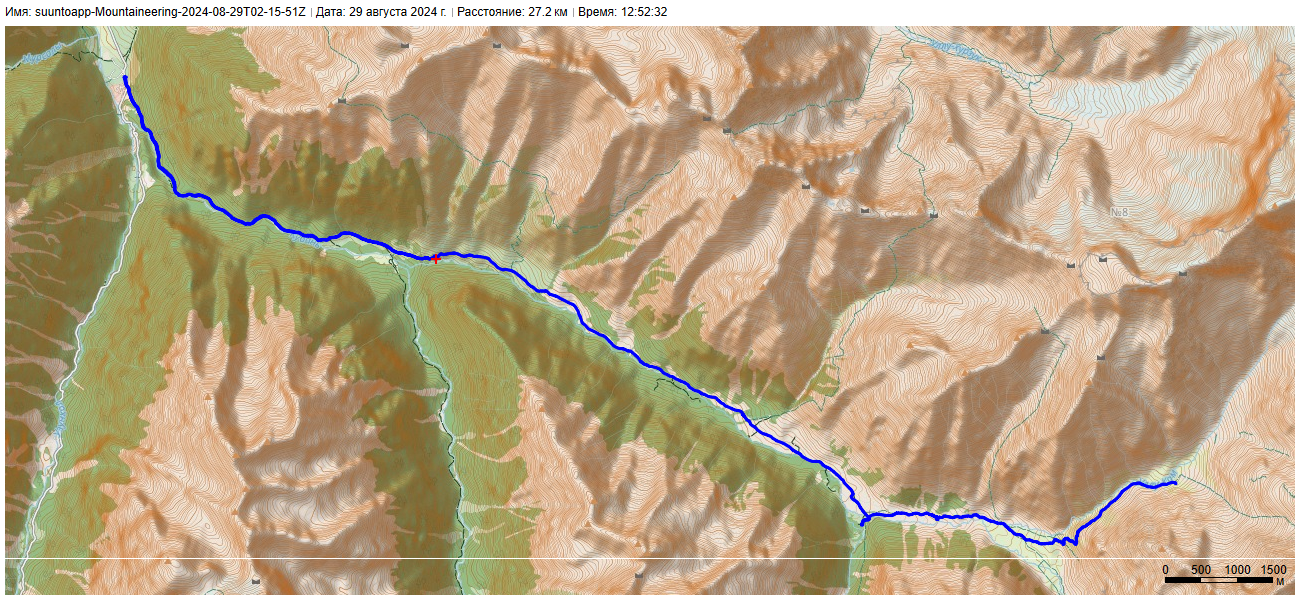
\includegraphics[angle=0, width=0.7\linewidth]{../pics/mini_maps/29}
	\label{fig:mini_29}
\end{figure}


Подъём руководов и части группы, которая сходит с маршрута (Дима Сингалевич, Илья, Даша Мерзликина, Маша) в 04:30. В 05:16 выходим вниз по д.р. Кубань. В 06:35 подходим к погранзаставе Актюбе-Хурзук. Необходимость сопровождения группы была обусловлена не только безопасностью, но и тем, что был оформлен групповой пропуск, и без заявителя группа не смогла бы покинуть погранзону. По пути обращаем внимание на синие метки трейлраннинговой тропы <<Alpindistria Elbrus Race>>.

В 08:30 возвращаемся в лагерь, где оставшаяся часть группы кормит нас завтраком, и выходим вверх по д.р. Кубань в 10:00.

\begin{figure}[h!]
	\centering
	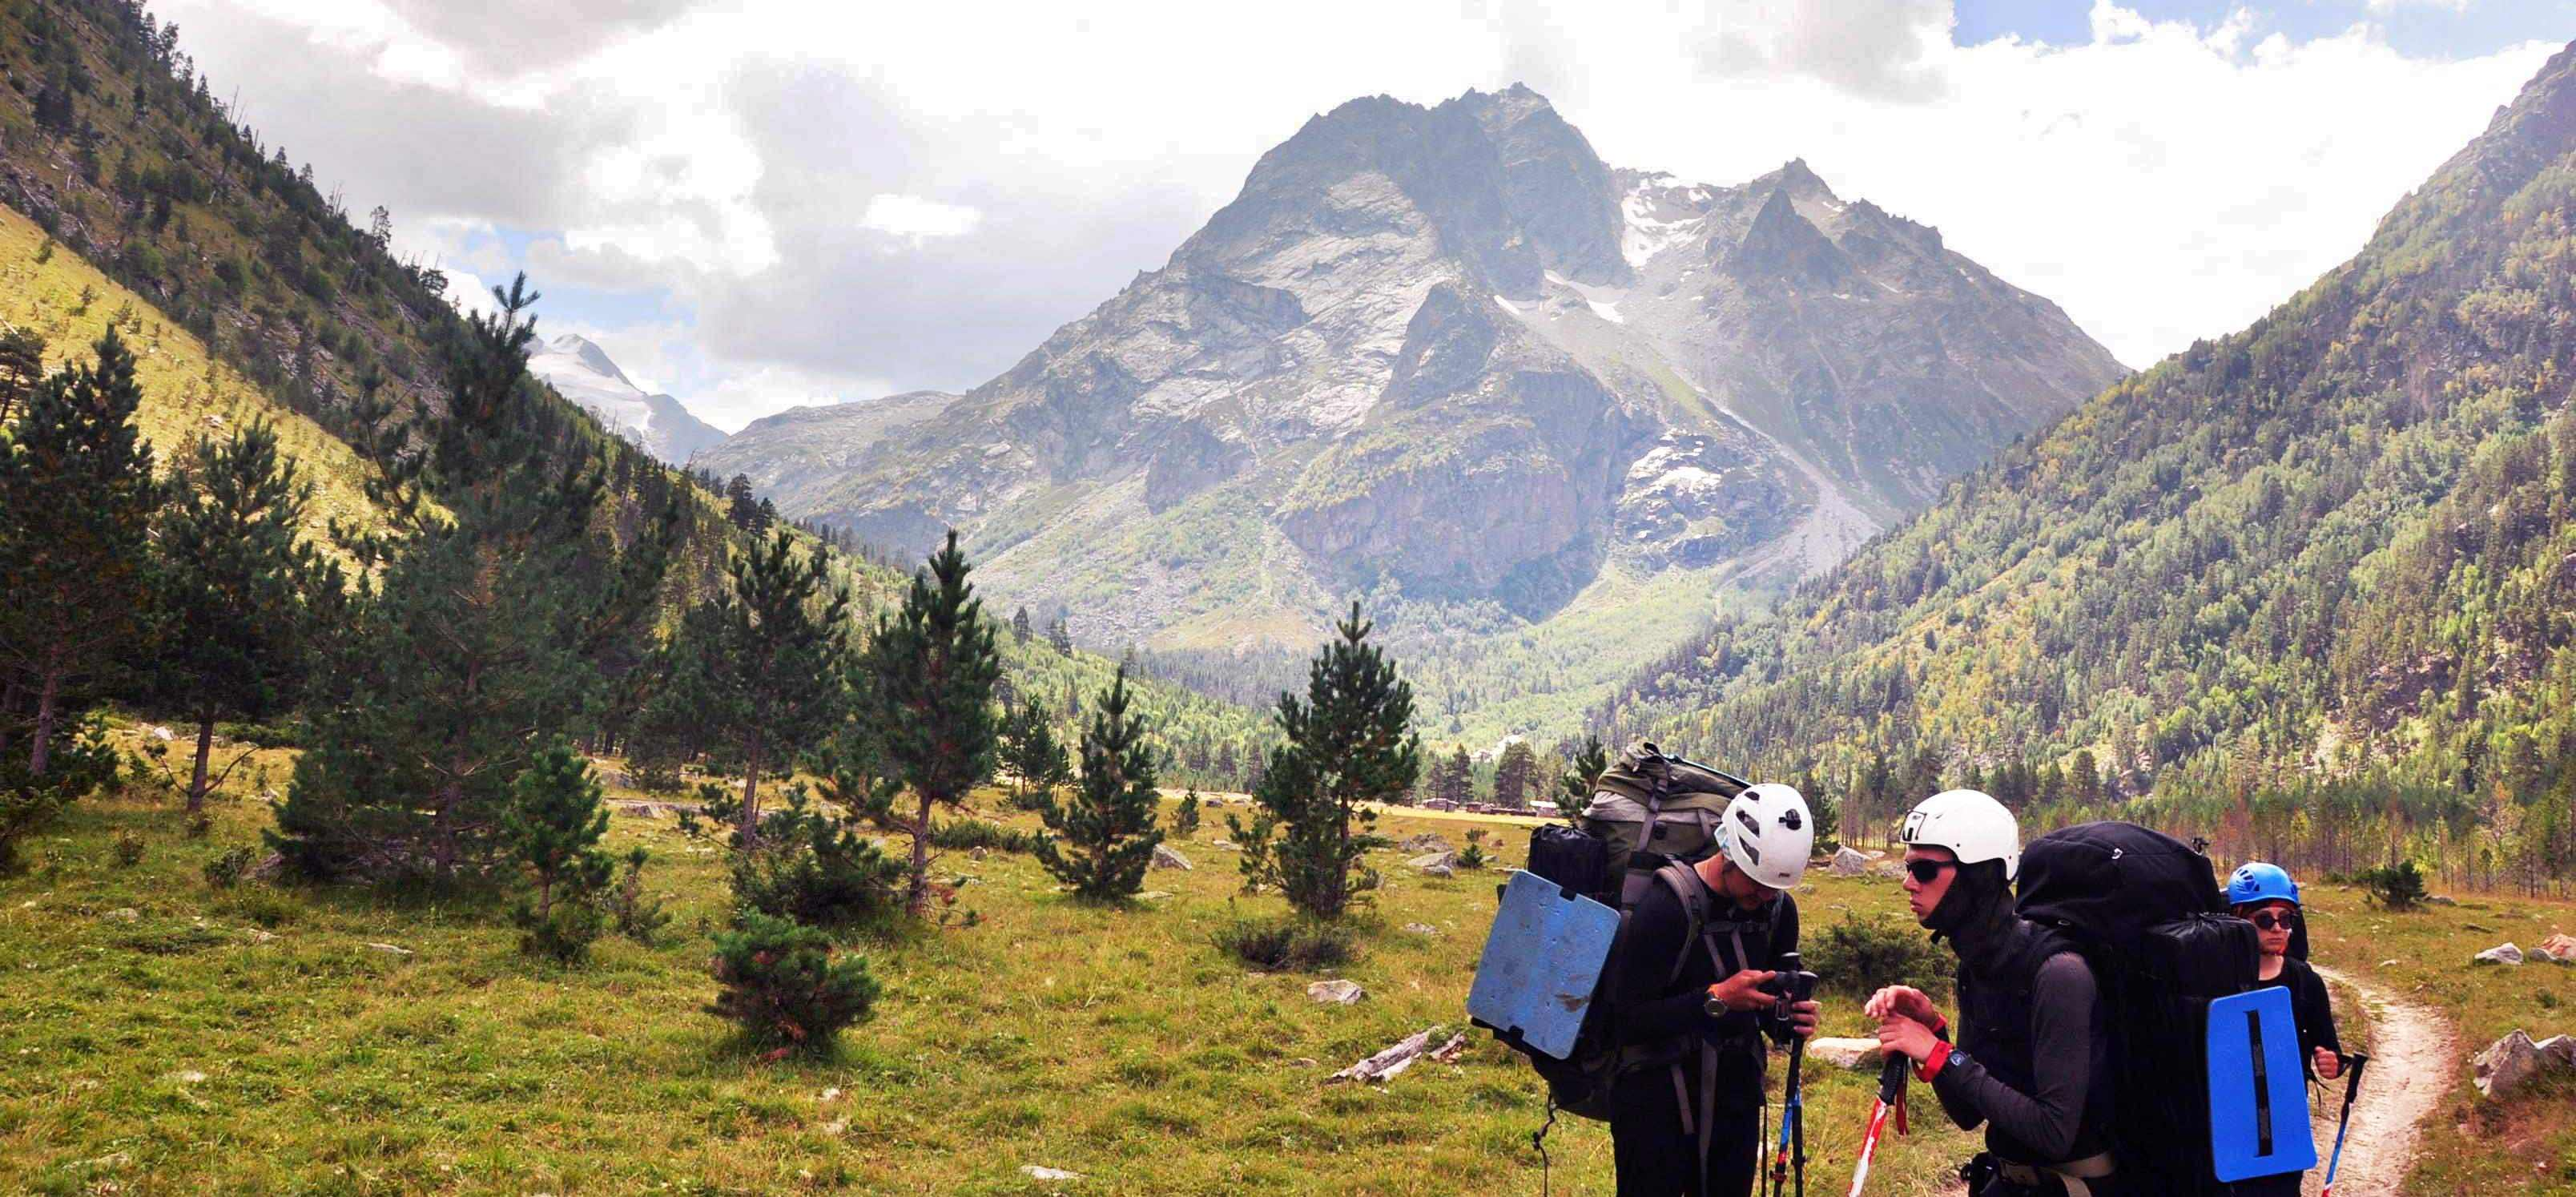
\includegraphics[width=0.7\linewidth]{../pics/DSC_0462 2.JPG}
	\caption{группа в д.р. Кубань}
	\label{fig:DSC_0462 2.JPG}
\end{figure}

Идём по хорошей автомобильной грунтовой дороге практически без набора высоты. Дорога идёт по открытой местности, иногда сменяется лесом (рис.~\ref{fig:DSC_0462 2.JPG}). Жарко, у ручьёв делаем привалы и набираем воду. Слева пхд тянутся каменные руины, предположительно, древних городищ.


В 12:50 доходим до Ворошиловских кошей, откуда сворачиваем направо пхд, к погранзаставе. Ждём пограничников 15 минут, но никто не откликается. Проходим немногим более 1~км вверх по течению р. Кубань и встаём на обед в 13:40 около небольшого ручья в тени деревьев, координаты места обеда N43.298154\degree,~E42.333682\degree. Во время нашего обеда к нам подходят два конных пограничника, интересуются нашим маршрутом, но документов не просят.

Выходим в 15:20, идём в сторону ущелья Уллу-Кам, ориентируемся, кроме прочего, на синие метки трейраннинговой тропы.

\begin{figure}[h!]
	\centering
	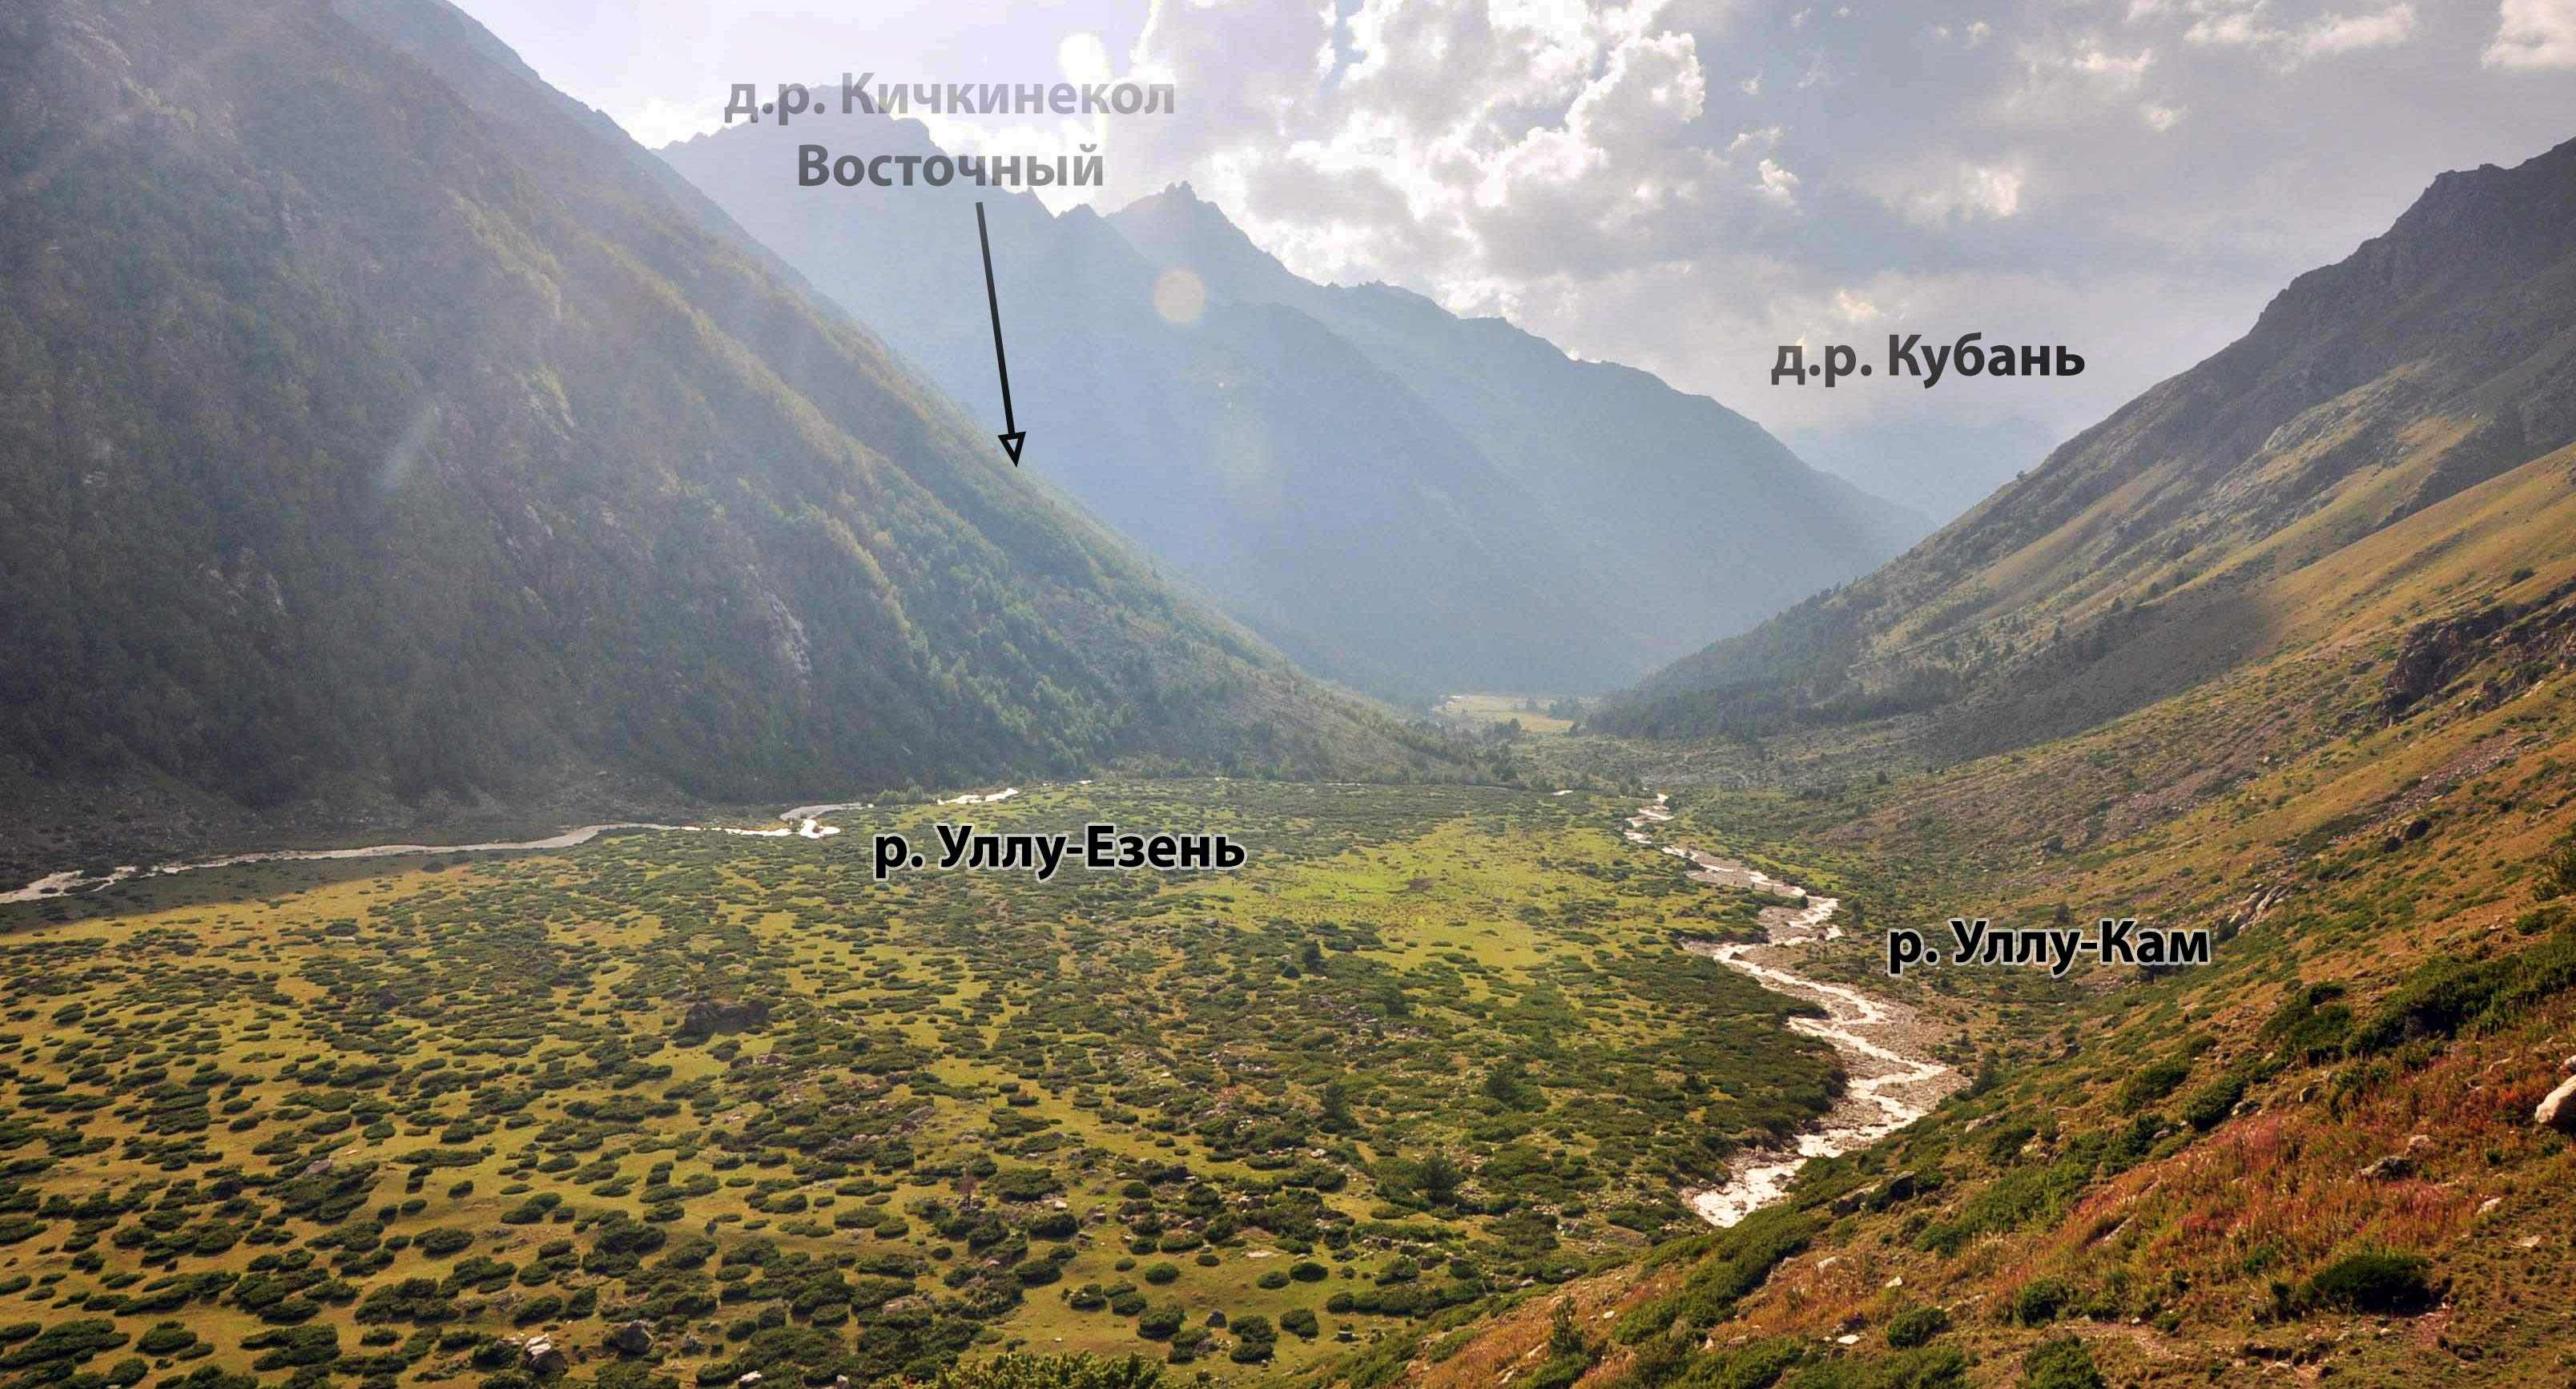
\includegraphics[width=0.7\linewidth]{../pics/DSC_0464 2.JPG}
	\caption{д.р. Кубань, вид с подъёма в д.р. Уллу-Кам}
	\label{fig:DSC_0464 2.JPG}
\end{figure}

После прохождения разлива рек Уллу-Кам и Уллу-Езень поворачиваем налево в ущелье Уллу-Кам. Начинаем подъём в 16:20. Тропа идёт по левому берегу реки, резко уходя вверх, затем пологим траверсом, выходя к берегу у оборудованного места ночёвки.


\begin{figure}[h!]
	\centering
	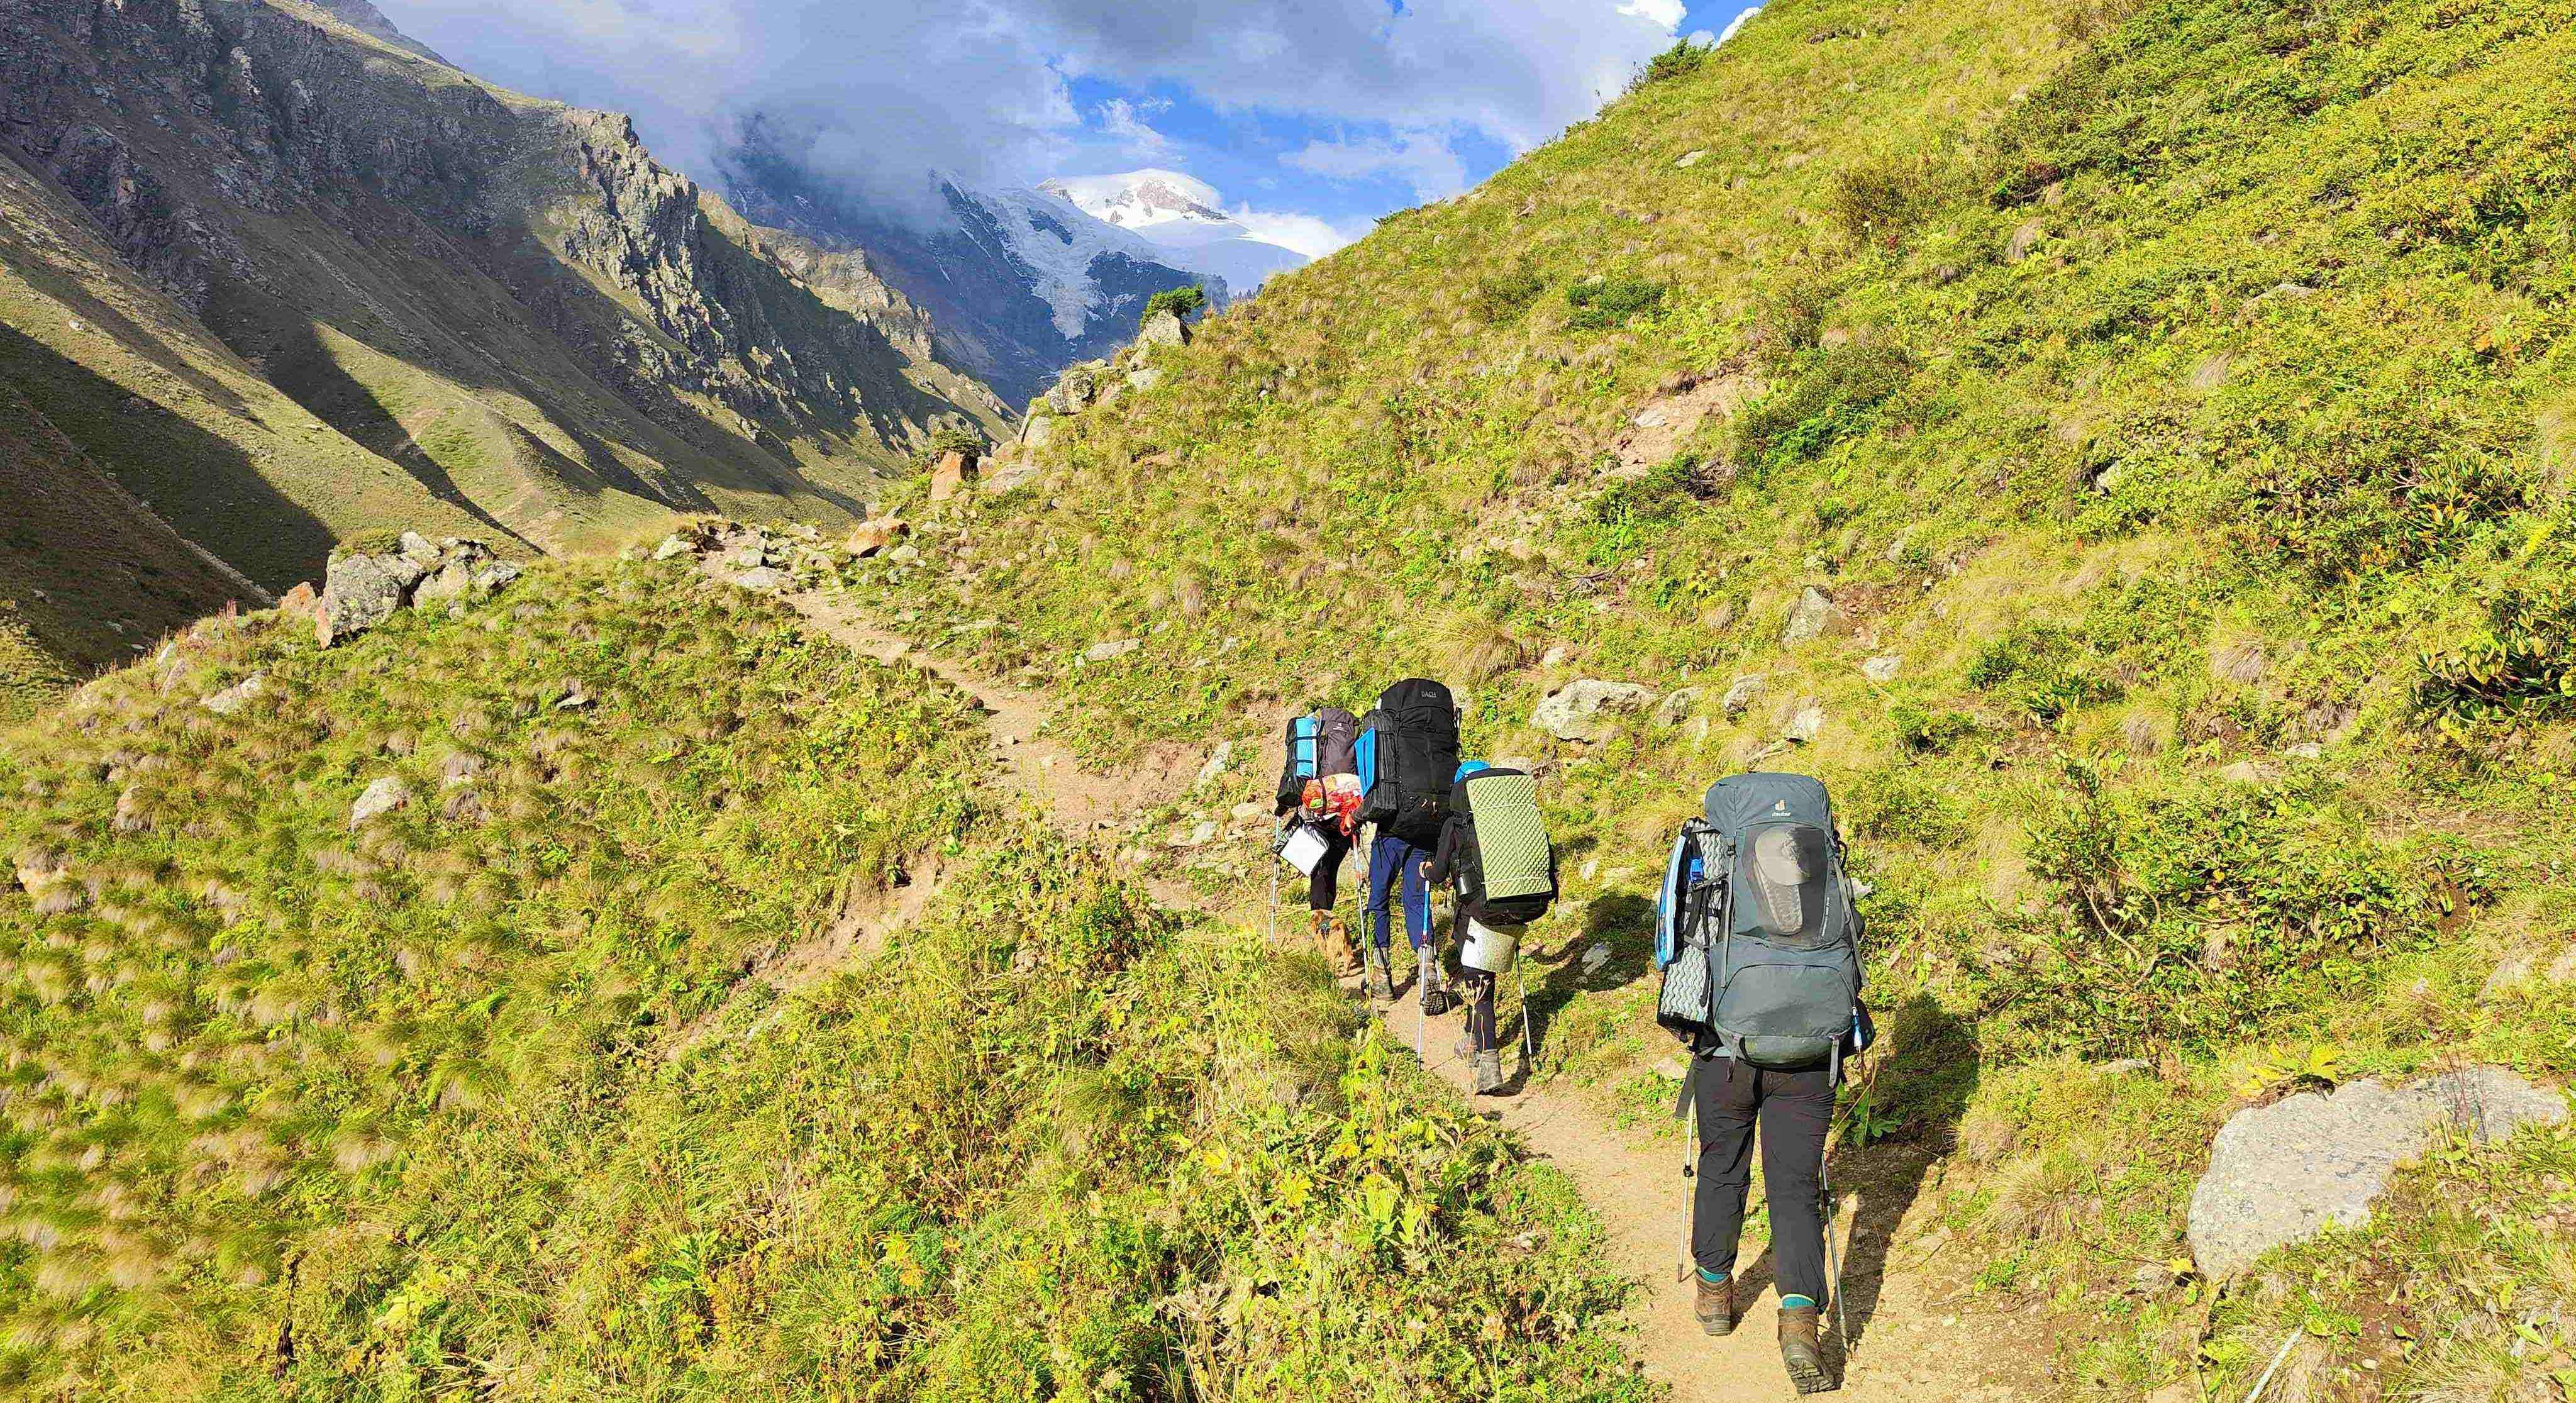
\includegraphics[width=0.7\linewidth]{../pics/IMG_20240829_170756.jpg}
	\caption{Тропа по траверсу}
	\label{fig:IMG_20240829_170756.jpg}
\end{figure}

За одним из поворотов нам открывается вид на юго-восточные скалы Эльбруса. Зрелище завораживающее: на переднем плане располагаются травяные горные склоны, на среднем плане они резко сменяются башнями Эльбруса из красной вулканической породы, а на дальнем плане~--- величественные снежные склоны.

\begin{figure}[h!]
	\centering
	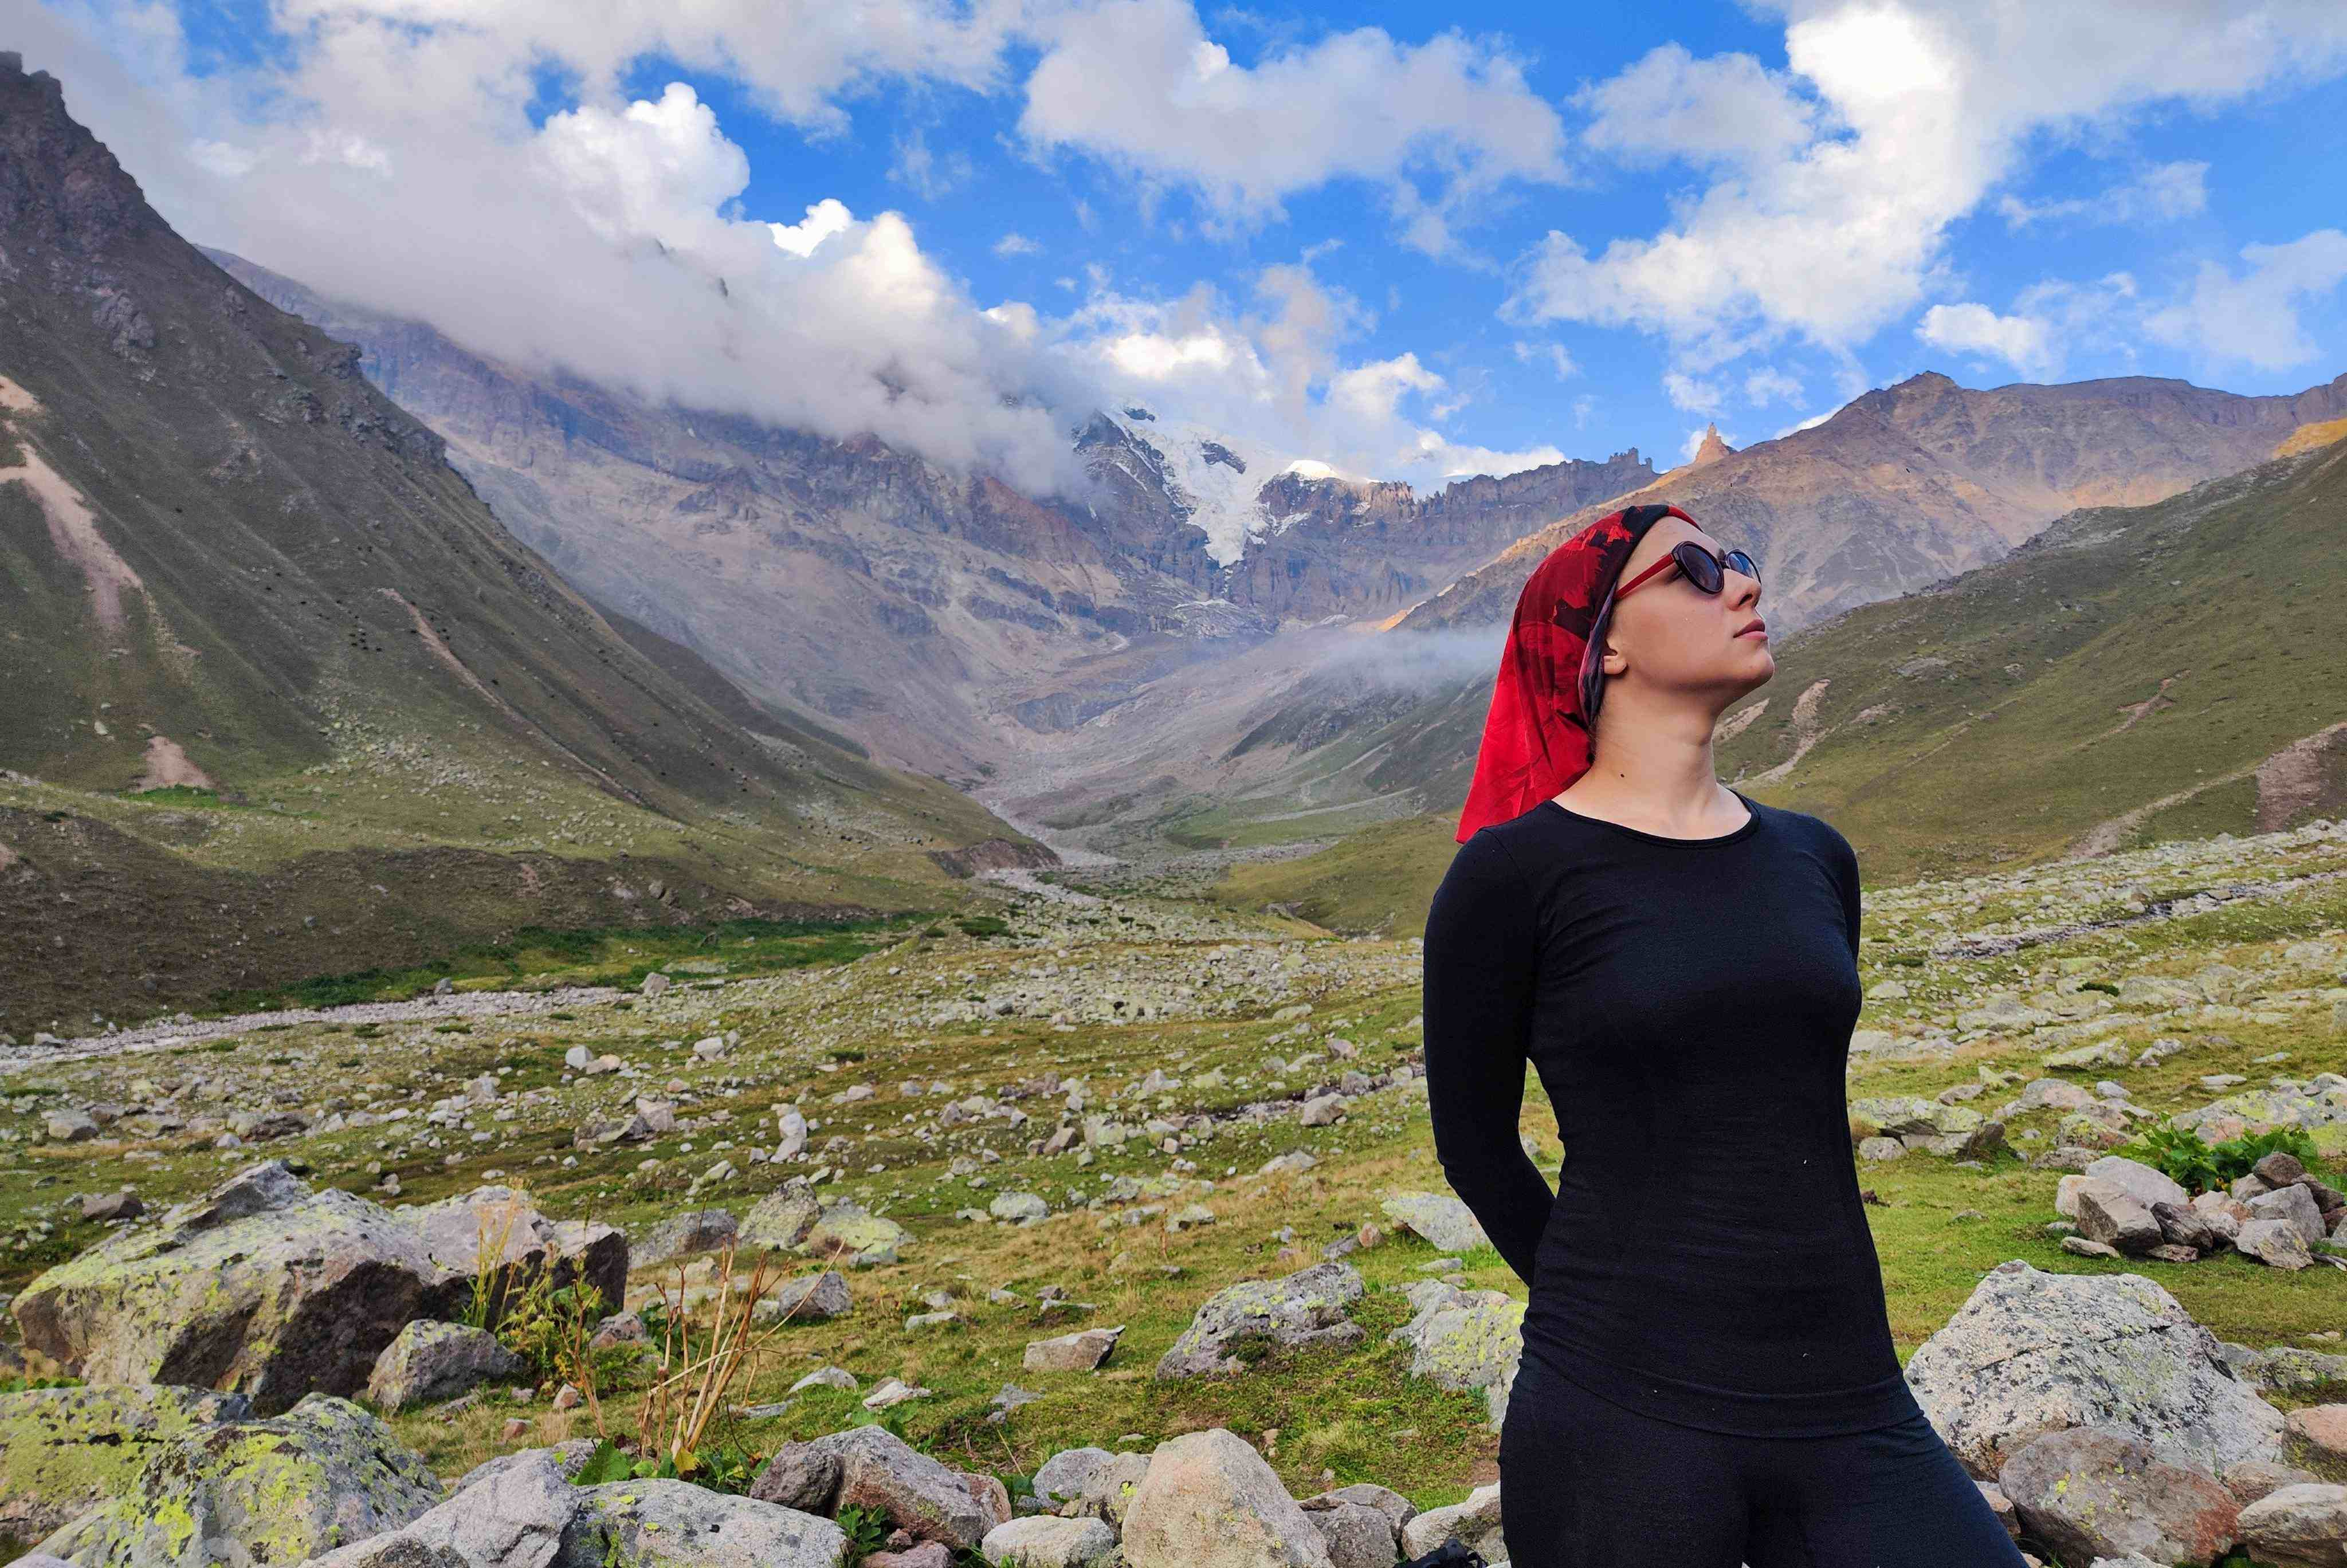
\includegraphics[width=0.7\linewidth]{../pics/IMG_20240829_181353.jpg}
	\caption{Вид на Эльбрус с м.н.}
	\label{fig:IMG_20240829_184033}
\end{figure}


\begin{figure}[h!]
	\centering
	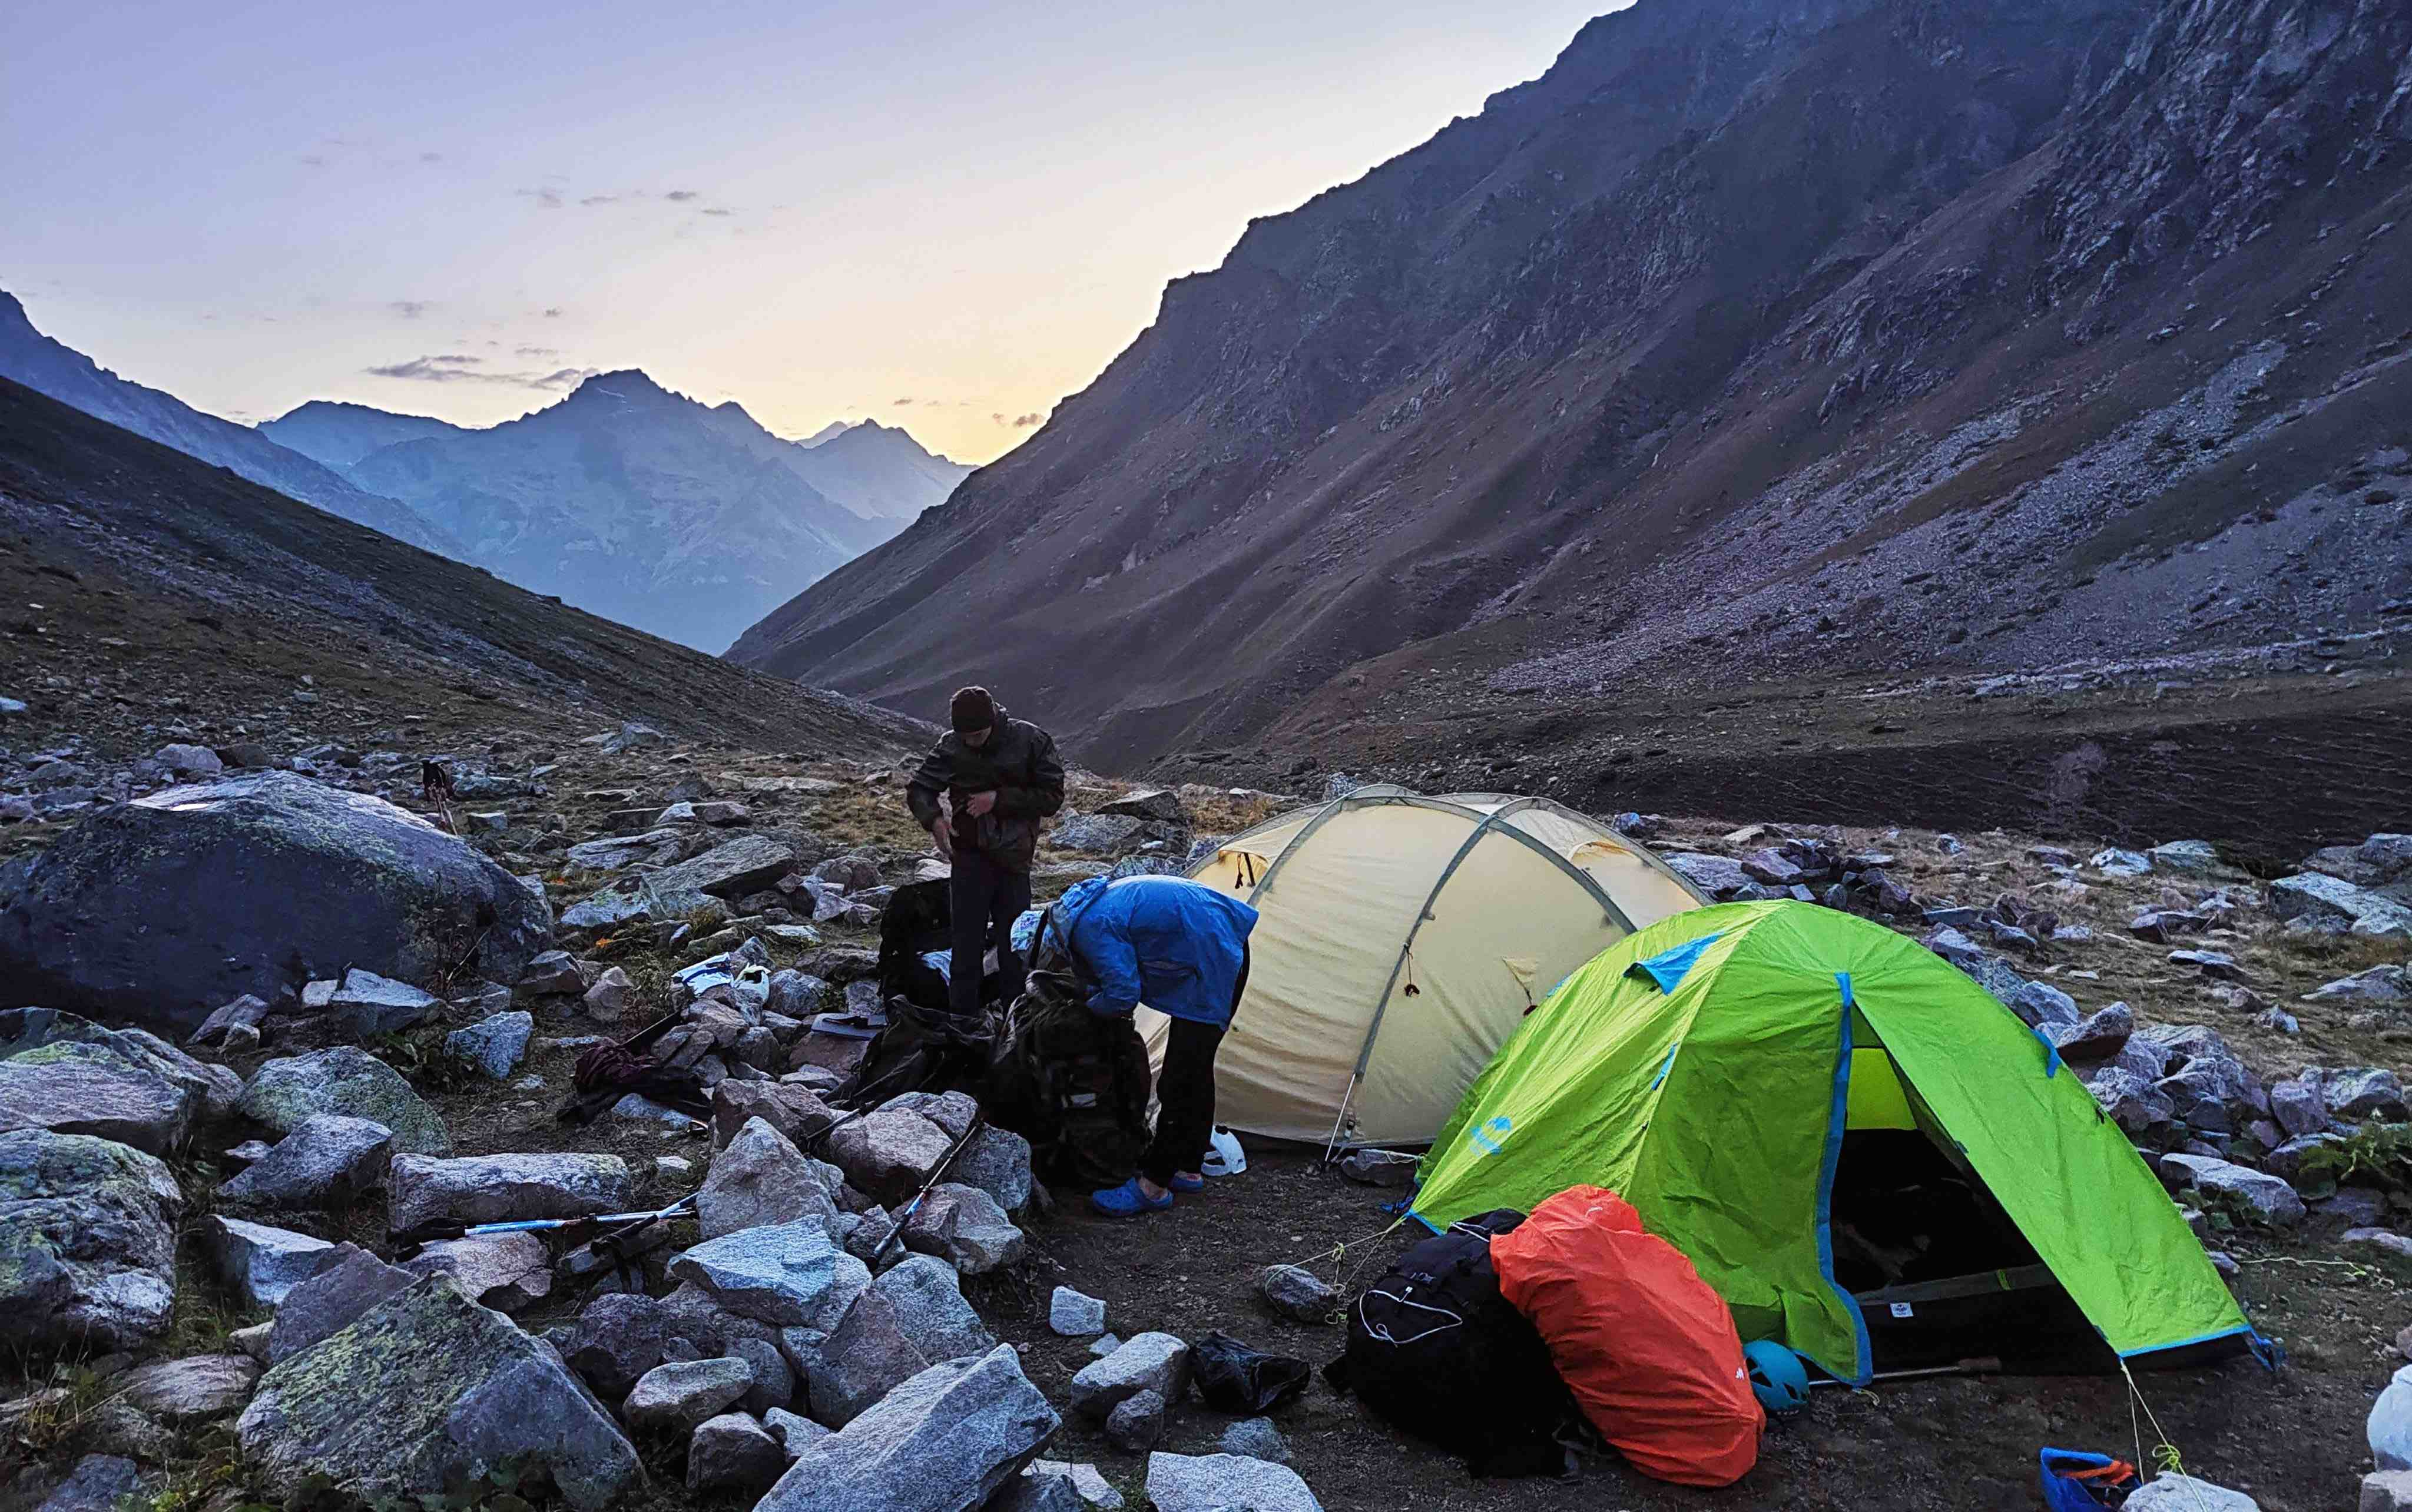
\includegraphics[width=0.7\linewidth]{../pics/IMG_20240829_191225.jpg}
	\caption{Место ночёвки 29-30 августа}
	\label{fig:IMG_20240829_191225.jpg}
\end{figure}

В 17:50 приходим на место ночёвки, есть расчищенные площадки под палатки. Открывается вид на Эльбрус, но быстро затягивается облаками. Коорлинаты м.н. N43.302568\degree, E42.374594\degree.


\clearpage